\documentclass{article}
% if you need to pass options to natbib, use, e.g.:
%     \PassOptionsToPackage{numbers, compress}{natbib}
% before loading neurips_2020

% ready for submission
% \usepackage{neurips_2020}

% to compile a preprint version, e.g., for submission to arXiv, add add the
% [preprint] option:
%     \usepackage[preprint]{neurips_2020}

% to compile a camera-ready version, add the [final] option, e.g.:
%     \usepackage[final]{neurips_2020}

% to avoid loading the natbib package, add option nonatbib:
\usepackage[preprint]{neurips_2020}
\usepackage[utf8]{inputenc} % allow utf-8 input
\usepackage[T1]{fontenc}    % use 8-bit T1 fonts
\usepackage{hyperref}       % hyperlinks
\usepackage{url}            % simple URL typesetting
\usepackage{booktabs}       % professional-quality tables
\usepackage{amsfonts}       % blackboard math symbols
\usepackage{nicefrac}       % compact symbols for 1/2, etc.
\usepackage{microtype}      % microtypography
\usepackage{multicol}
\usepackage{xeCJK}
\usepackage{subfigure}
\usepackage{tabularx}
\usepackage{graphicx}
\usepackage{indentfirst}
\setlength{\parindent}{2em}

\title{Principles of Data Science Project 1\\
        Dimension Reduction}

% The \author macro works with any number of authors. There are two commands
% used to separate the names and addresses of multiple authors: \And and \AND.
%
% Using \And between authors leaves it to LaTeX to determine where to break the
% lines. Using \AND forces a line break at that point. So, if LaTeX puts 3 of 4
% authors names on the first line, and the last on the second line, try using
% \AND instead of \And before the third author name.

\author{
  Hongzhou Liu \\
  517030910214 \\
  \texttt{deanlhz@sjtu.edu.cn} \\
  \And
  Xuanrui Hong \\
  517030910227 \\
  \texttt{aaa@bbb.ccc} \\
  \And
  Qilin Chen \\
  517030910155 \\
  \texttt{1017856853@sjtu.edu.cn} \\
}

\newcommand{\fix}{\marginpar{FIX}}
\newcommand{\new}{\marginpar{NEW}}

\begin{document}
\bibliographystyle{unsrt}

\maketitle

\textbf{To Xuanrui Hong:}\\
请先完成Method部分\\
截止日期:周六晚24点\\
提交方式:\texttt{git}\\
\begin{itemize}
  \item 可以使用ppt上的图片、公式,使用公式必须要完整体现这个方法的内涵
  \item 可以参考维基百科,但需要做一定的改写, i.e. paraphrase
  \item 参考文献获取途径:前往\texttt{sci-kit learn}官方网站,搜索对应的方法,如PCA,在相应文档页面查找是否有参考文献。或者找到左上角User Guide,寻找相应内容,如2.Unsupervised Learning-2.5.Decomposing signals in components (matrix factorization problems)
  \item 可以参考往届报告,行文风格、参考文献等,但不必每个方法处处都引用
\end{itemize}

\textbf{To Qilin Chen:}\\
请完成Experiement中Feature Selection之外的部分及Conclusion部分(周日晚Xuanrui Hong会完成Feature Selection部分的分析,并\texttt{push}至仓库中,请使用\texttt{git pull}获取)
截止日期:周二晚24点 \\
提交方式:\texttt{git} \\
\begin{itemize}
  \item 所有实验结果均在Prj1/Result下,包括不同方法、不同维度的降维结果用线性SVM以及核SVM(RBF核)的分类精度(文本、点线图),以及2维降维结果的可视化(训练集、测试集)
  \item Baseline已经给出,请以baseline为基准比较各方法结果
  \item 请恰当使用\texttt{figure}、\texttt{subfigure}等方式美观地排版图片
  \item 请正确地设计表格,以表现不同降维方法、不同分类器(线性SVM以及核SVM)产生的结果变化,并突出最佳参数设置
  \item AutoEncoder部分请查看代码(Prj1/Projection/AutoEncoder.py)获取神经网络结构、超参数等数据,并在文中体现
  \item 关于参考文献:前往\texttt{sci-kit learn}官方网站,搜索对应的方法,如PCA,在相应文档页面查找是否有参考文献。或者找到左上角User Guide,寻找相应内容,如2.Unsupervised Learning-2.5.Decomposing signals in components (matrix factorization problems)。除此之外还可以寻找其他参考文献。
  \item 可以参考往届报告,行文风格、参考文献等
  \item 请修改上方\texttt{author}部分你的邮箱
  \item 由于是多人同时完成不同的部分,每次修改前请使用\texttt{git pull}保持与远程仓库的同步,修改完毕后及时使用\texttt{git push}
\end{itemize}

\begin{abstract}
  TODO: Hongzhou Liu\\
\end{abstract}

\section{Method}
\subsection{Feature Selection}
\subsubsection{Select-k-best}
\indent SelectKBest is one of the methods of univariate feature selection, which works by selecting the best features based on univariate statistical tests. It removes all but the $k$ highest scoring features.
\subsubsection{Variance Threshold}
\indent VarianceThreshold is a simple approach to feature selection. It removes all features whose variance doesn’t meet some threshold. The principle is that features with small variance often contain less data information.
\subsubsection{Tree-based Selection}
\indent Tree-based feature selection combines SelectFromModel and ExtraTreesClassifier. SelectFromModel is a meta-transformer that can be used along with any estimator that has a $coef\_$ or $feature\_importances\_$ attribute after fitting. The features whose $coef\_$ or $feature\_importances\_$ values are below the provided threshold parameterare are considered unimportant and removed. ExtraTreesClassifier can be used to compute feature importances, which happens to cooperate with SelectFromModel to discard irrelevant features.

\subsection{Feature Projection}
\subsubsection{PCA}
\indent Principal component analysis is one of the most widely used data dimensionality reduction algorithms. It performs a linear mapping of the data to a lower-dimensional space in such a way that the variance of the data in the low-dimensional representation is maximized.\cite{pearson1901liii}
Formally, the optimization goal is
\begin{eqnarray}
\centering
\max_v \frac{1}{n}\sum_{i=1}^{n}(v^Tx_i)^2=\frac{1}{n}v^TXX^Tv
\end{eqnarray}
where $v$ is the new axis.
\begin{eqnarray}
s.t.\quad v^Tv=1
\end{eqnarray}
Using lagrange Multiplier we can get
\begin{eqnarray}
XX^Tv=\lambda v
\end{eqnarray}
We can see that $v$ is the eigenvector of $XX^T$, and $\lambda$ is the corresponding eigenvalue. Therefore, $v$ can be calculated by performing eigenvalue decomposition to the co-variance matrix $XX^T$. Then we can get the data after dimensionality reduction.
\subsubsection{Kernel PCA}
\indent In general, principal components analysis is suitable for linear dimensionality reduction of data. Kernel PCA can achieve nonlinear dimensionality reduction of data and is used to process linear inseparable data sets.\\
\indent The general idea of KPCA is: for the matrix in the input space, we first use a non-linear mapping to map all samples in a high-dimensional or even infinite-dimensional space, and then perform PCA dimensionality reduction in this high-dimensional space.
\subsubsection{LDA}
\indent Linear discriminate analysis is commonly used as dimensionality reduction technique. Its main idea is to project the samples on a straight line so that the projections of similar samples are as close as possible, and the projection points of heterogeneous samples are as far as possible. 
	\begin{figure}[htbp]
		\centering
		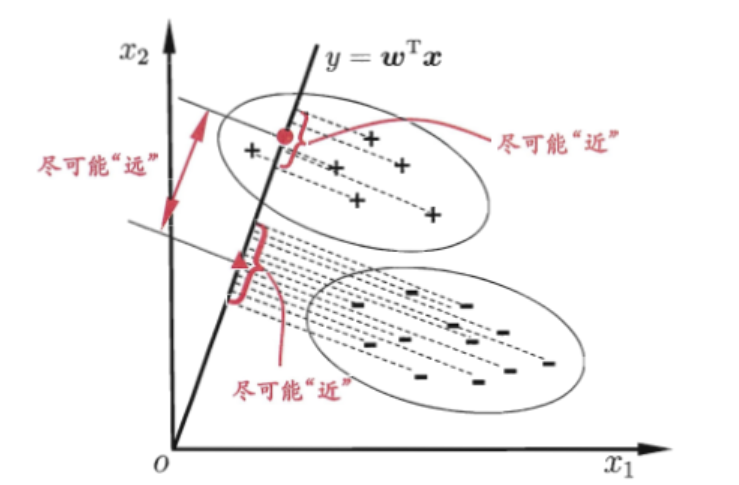
\includegraphics[scale=0.3]{figures/LDA.png}
		\caption{Two-dimensional illustration of LDA.}
		\label{fig:LDA}
	\end{figure}\cite{zhihuazhou2016ml}\par
\indent The key step of LDA:
\begin{itemize}
		\item Standardize d-dimensional data (d is the number of features).
		
		\item For each category, calculate the d-dimensional mean vector.
		
		\item Construct inter-class scatter matrix $S_B$ and intra-class scatter matrix $S_W$.
		
		\item Calculate the eigenvalues and corresponding eigenvectors of the matrix $S^{-1}_WS_B$.
		
		\item Select the eigenvectors corresponding to the first $k$ eigenvalues to construct a $d × k$ dimension transformation matrix $W$, where the eigenvectors are arranged in columns.
		
		\item Use the transformation matrix $W$ to map the samples to the new feature subspace.
		
\end{itemize}
\subsubsection{AutoEncoder}
\indent An autoencoder is a type of artificial neural network used to learn efficient data codings in an unsupervised manner.\cite{kramer1991nonlinear}The purpose of autoencoder is to train a neural network for sample dimensionality reduction, and the sample after dimensionality reduction can reconstruct the original sampel well. \par
\indent It contains encoder and decoder. The coding network belongs to the dimension reduction part, and the role is to reduce the high-dimensional original data to a low-dimensional nested structure with a certain number of dimensions; the decoding network belongs to the reconstruction part, which can be regarded as the reverse process of the coding network. There is also an intersection between the encoding network and the decoding network, called the "code layer", which is the core of the entire self-encoding network  and can determine the essential dimensions of high-dimensional datasets.
\begin{figure}[htbp]
	\centering
	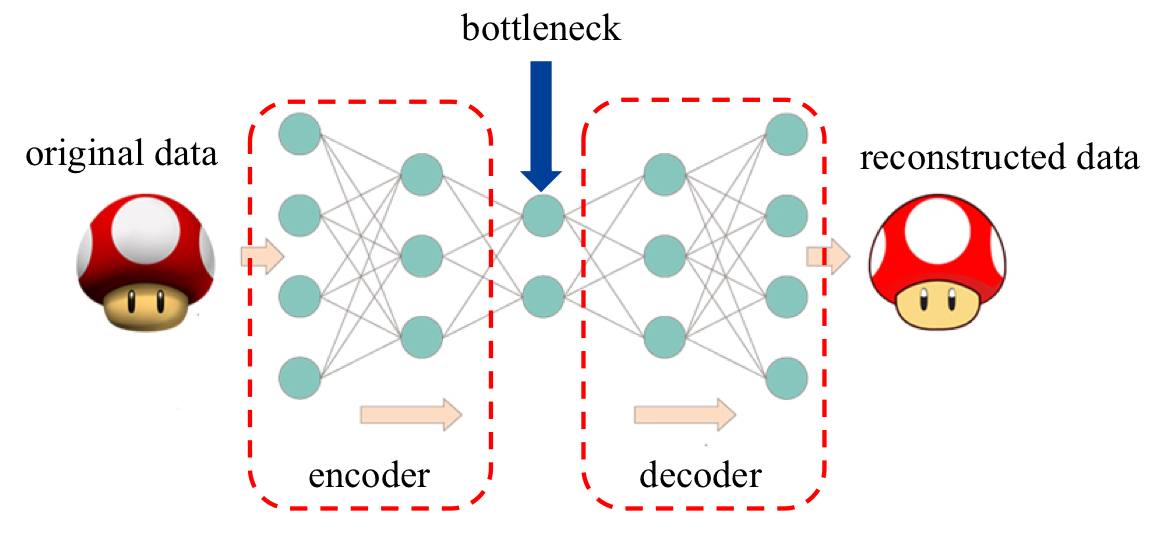
\includegraphics[scale=0.2]{figures/Autoencoder.jpg}
	\caption{Autoencoder.}
	\label{fig:autoencoder}
\end{figure}\par
\subsection{Feature Learning}
\subsubsection{t-SNE}
\indent T-distributed stochastic neighbor embedding is a machine learning algorithm for dimensionality reduction, proposed by Laurens van der Maaten and Geoffrey Hinton in 2008.\cite{maaten2008visualizing}It is a nonlinear dimensionality reduction technique. T-SNE obtains $\tilde{x}$ from $x$ and maintains the relative distance as much as possible. Its main steps are:
\begin{itemize}
	\item  Evaluate the similarity of data point $x_i$ and data point $x_j$ by
	\begin{eqnarray}
	p_{j|i}=\frac{(1+\Vert x_i-x_j \Vert^2)^-1}{\sum_{k\neq i}(1+\Vert x_i-x_k \Vert^2)^-1}
	\end{eqnarray}
	
	\item  Meature similarity of data point $\tilde{x_i}$ and data point $\tilde{x_j}$ by
	\begin{eqnarray}
	q_{j|i}=\frac{(1+\Vert \tilde{x_i}-\tilde{x_j} \Vert^2)^-1}{\sum_{k\neq i}(1+\Vert \tilde{x_i}-\tilde{x_k} \Vert^2)^-1}
	\end{eqnarray}
	
	\item  Minimize the $Kullback-Leibler divergence$ of the distribution $Q$ from the distribution $P$, that is
	\begin{eqnarray}
	L = \sum_{i}KL(P_i\Vert Q_i)=\sum_{i}\sum_{j}p(i|j)log\frac{p_{j|i}}{q_{j|i}}
	\end{eqnarray}
\end{itemize}

\indent Besides, t-SNE is the deformation of SNE. The difference is that t-SNE uses t-distribution while SNE uses Gaussian distribution.
\begin{figure}[htbp]
	\centering
	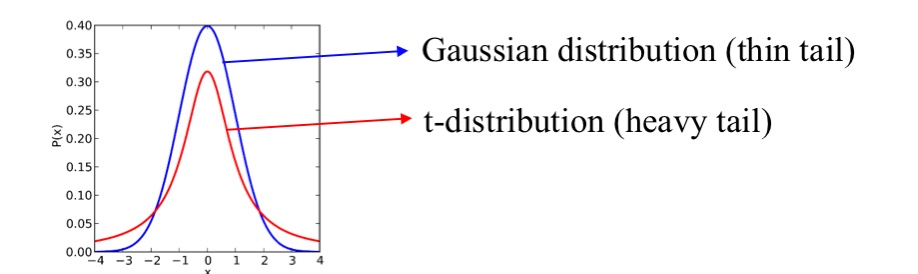
\includegraphics[scale=0.3]{figures/SNE.jpg}
	\caption{t-SNE and SNE.}
	\label{fig:SNE}
\end{figure}\par

\subsubsection{LLE}
Locally Linear Embedding (LLE) is a member of the manifold learning algorithm and is a nonlinear dimensionality reduction method. LLE was invented in 2000 and published in the journal Sience.\cite{roweis2000nonlinear}LLE algorithm tries to maintain the linear relationship between samples in the neighborhood. As shown in figure 3,the sample $x_i$ in the high-dimensional space can be reconstructed from its neighbor sample $x_j,x_k,x_l$ through linear combination, ie
\begin{eqnarray}
x_i = w_{ij}x_j+w_{ik}x_k+x_{il}x_l
\end{eqnarray}
\begin{figure}[htbp]
	\centering
	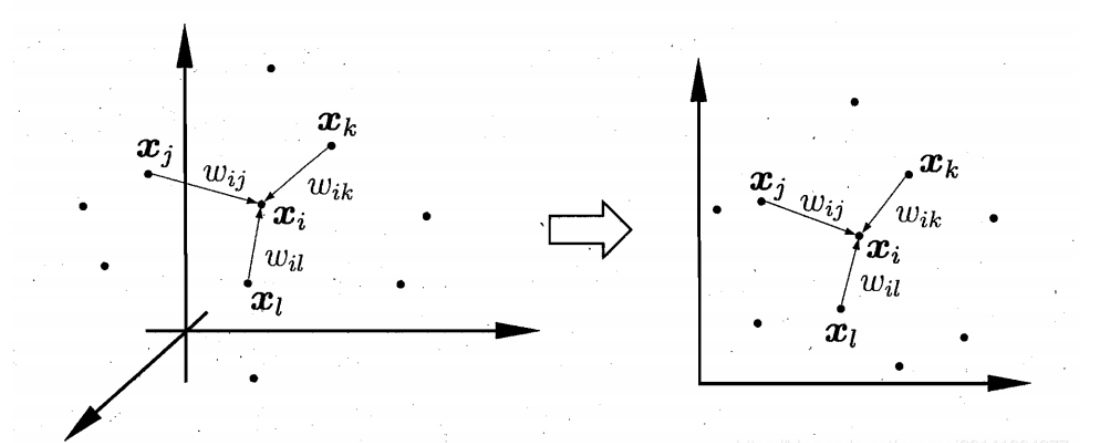
\includegraphics[scale=0.3]{figures/LLE.png}
	\caption{LLE.}
	\label{fig:LLE}
\end{figure}\par
\indent Its main steps are:
\begin{itemize}
	\item Learn the linear relation $W$ between each sample and its neighbors, which can be formalized as:
	\begin{eqnarray}
	W = \mathop{\arg\min}_{W}\sum_{i=1}^{m}\Vert x_i-\sum_{j\in N(i)}w_{ij}x_j\Vert^2 
	\end{eqnarray}
	where $N(i)$ is the k-nearest neighbors of $x_i$
	
	\item  Reconstruct the low-dimensional features:
	\begin{eqnarray}
	Z = \mathop{\arg\min}_{Z}\sum_{i=1}^{m}\Vert z_i-\sum_{j\in N(i)}w_{ij}z_j\Vert^2 
	\end{eqnarray}
	where $z_i$ is the sample after dimensionality reduction of $x_i$
\end{itemize}

\section{Experiment}
\subsection{Baseline}
TODO: Hongzhou Liu\\
Training Set : Test Set = 6:4 \\
Linear SVM: Best C = 0.002, best accuracy = 0.932815 (baseline) \\
Kernel SVM with RBF kernel: Best C = 5.0, best accuracy = 0.935160 (baseline) \\
\subsection{Feature Selection}
\subsubsection{Select-k-best}
TODO: Xuanrui Hong\\
\subsubsection{Variance Threshold}
TODO: Xuanrui Hong\\
\subsubsection{Tree-based Selection}
TODO: Xuanrui Hong\\

\subsection{Feature Projection}
\subsubsection{PCA}
Principal component analysis (PCA) is the most typical feature projection method based on dimension reduction, since PCA provides a roadmap for how to reduce a complex data set to a lower dimension to reveal the sometimes hidden, simplified dynamics that often underlie it. Kernel principal component analysis (kernel PCA) provides an extension of traditional PCA using techniques of kernel methods, which project source data into a higher dimensional space, providing with better reduction and classification performance. In this section, two experiment settings can derive from the rule: We use kernel PCA on different number of aim component $[2, 5, 10, 20, 50, 100, 200, 500, 750, 1000, 1200, 1500, 2000]$, and we give our results on two types of kernel: linear kernel and radial basis function kernel. We adopt classifiction accuracy as metric in this section.

We summarize the experimental results of kernel PCA in Tab. \ref{baseline1} and Fig. \ref{Fig1}. As is shown, linear kernel PCA model and RBF kernel PCA model expectively exhibit the best performances at 200 components and 750 components, reaching $92.20\%$ and $92.50\%$ on the classification task. We can compare the result with the simple linear SVM and simple RBF SVM, find the kernel PCA model's performance is worse than the baselines, and we deem the reason is that compoents reduction of PCA remove some effective feature as it remove the most noisy feature. And we can find RBF kernel have better performance than linear kernel in PCA tasks and none-PCA tasks, it proves the provided dataset have some features which can't be handled merely by linear kernel. Besides, in kernel PCA tasks, we can find if we have less components, RBF kernel have better performance than linear kernel.

We give the 2-components scattering figure of different kernel and dataset in Fig. \ref{Fig2}, which can support the result that RBF kernel have better performance than linear kernel since the RBF figure can be better splited. What's more, if we compare the trainset and testset, we can find the dataset is randomly splited.

\begin{table}
	\centering
	\newcommand{\tabincell}[2]{\begin{tabular}{@{}#1@{}}#2\end{tabular}}
	\renewcommand\arraystretch{1.1}
	\caption{Comparison of kernel PCA and baslines in Classification Task}
	\label{baseline1}%
	\resizebox{\linewidth}{!}{
	\begin{tabular}{c|c|c|c|c}
		\hline
		Model &\multicolumn{2}{c|}{PCA+SVM}&\multicolumn{2}{c}{SVM}\\
		\hline
		{components number} & {Linear kernel(\%)} & {RBF kernel(\%)}& {Linear kernel(\%)} & {RBF kernel(\%)}\\
		\cline{2-5}
		\hline
		2   & 12.46 & 19.68 & 93.28 & 93.52\\
		\hline
		5   & 40.31 & 59.68 & 93.28 & 93.52\\
		\hline
		10   & 68.99 & 78.25 & 93.28 & 93.52\\
		\hline
		20   & 82.27 & 87.07 & 93.28 & 93.52\\
		\hline
		50  & 89.31 & 90.53 & 93.28 & 93.52\\
		\hline
		100  & 91.37 & 91.66 & 93.28 & 93.52\\
		\hline
		200  & 92.20 & 91.94 & 93.28 & 93.52\\
		\hline
		500  & 92.14 & 92.42 & 93.28 & 93.52\\
		\hline
		750  & 91.90 & 92.50 & 93.28 & 93.52\\
		\hline
		1000  & 91.70 & 92.44 & 93.28 & 93.52\\
		\hline
		1200  & 91.78 & 92.26 & 93.28 & 93.52\\
		\hline
		1500  & 91.57 & 91.85 & 93.28 & 93.52\\
		\hline
		2000  & 91.64 & 88.08 & 93.28 & 93.52\\
		\hline
	\end{tabular}}
\end{table}

\begin{figure}
\centering
\subfigure[metric accuracy comparison on linear PCA]{
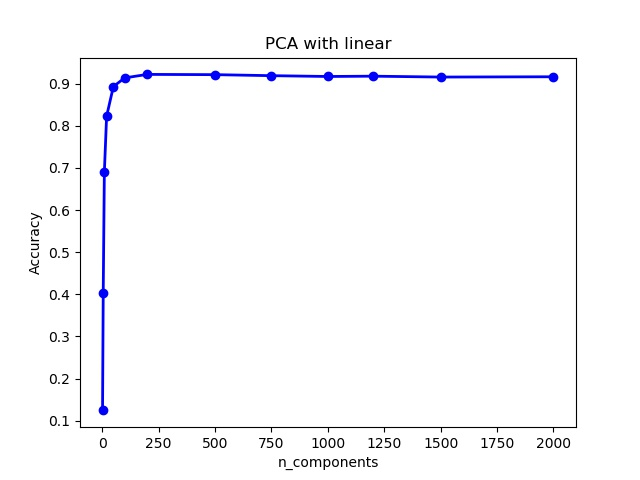
\includegraphics[width=6.5cm]{figure/PCA_linear.jpg}
%\caption{fig1}
}
\quad
\subfigure[metric accuracy comparison on RBF PCA]{
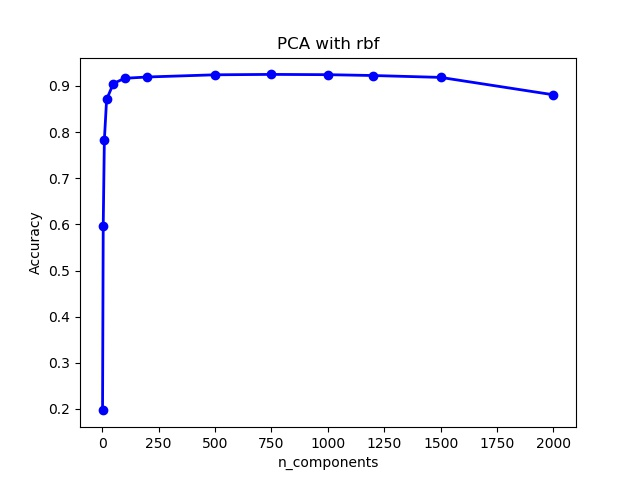
\includegraphics[width=6.5cm]{figure/PCA_rbf.jpg}
}
\caption{Kernel PCA performance on linear kernel and RBF kernel}
\label{Fig1}
\end{figure}

\begin{figure}
\centering
\subfigure[Trainset 2D scatter with linear PCA]{
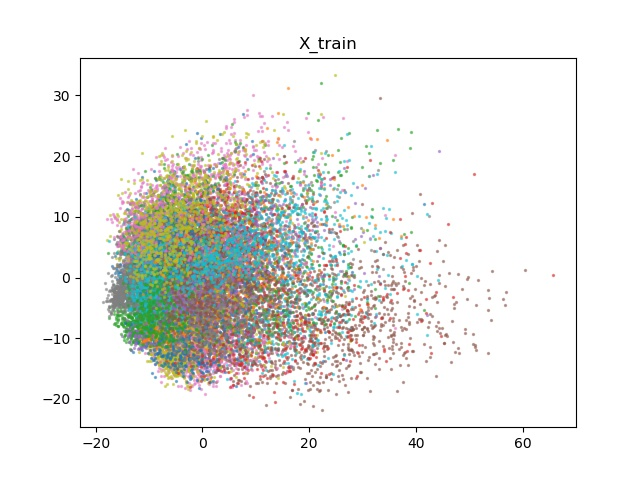
\includegraphics[width=6.5cm]{figure/X_train_scatter_2d_linear.jpg}
%\caption{fig1}
}
\quad
\subfigure[Testset 2D scatter with linear PCA]{
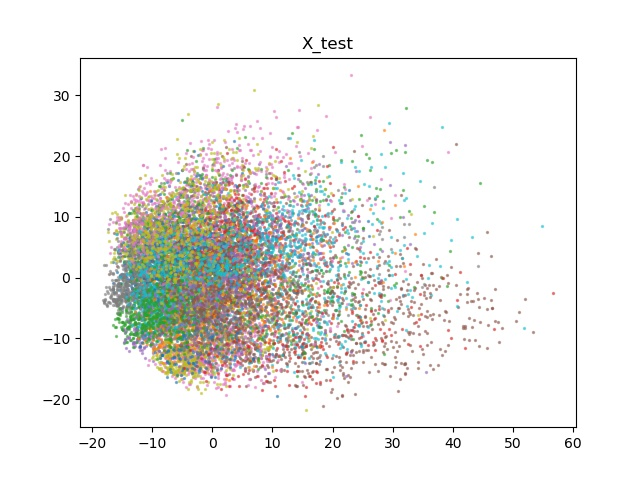
\includegraphics[width=6.5cm]{figure/X_test_scatter_2d_linear.jpg}
}
\quad
\subfigure[Trainset 2D scatter with RBF PCA]{
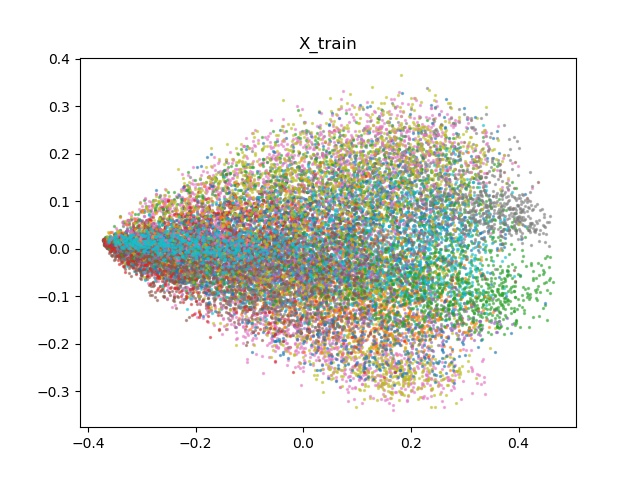
\includegraphics[width=6.5cm]{figure/X_train_scatter_2d_rbf.jpg}
}
\quad
\subfigure[Testset 2D scatter with RBF PCA]{
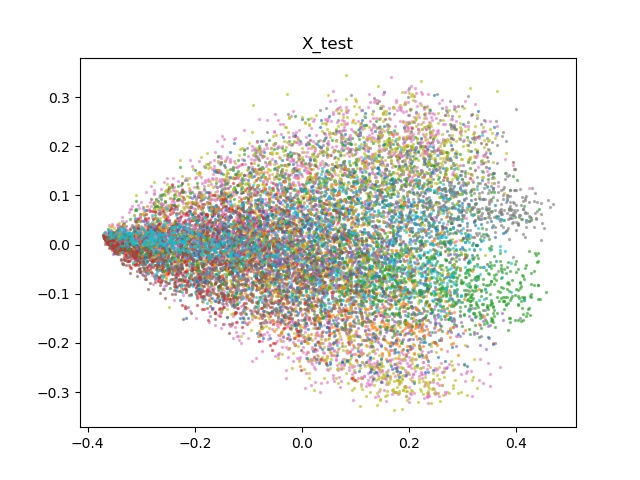
\includegraphics[width=6.5cm]{figure/X_test_scatter_2d_rbf.jpg}
}
\caption{Dataset 2D scatter with linear kernel and RBF kernel}
\label{Fig2}
\end{figure}

\subsubsection{LDA}

Linear discriminate analysis (LDA) is a dimension reduction technique that is closely related to principal component analysis (PCA) and factor analysis in that they both look for linear combinations of variables which best explain the data. However, in contrast, LDA explicitly attempts to model the difference between the classes of data. In this section, we use LDA model to project features into [2, 3, 5, 10, 20, 30, 40] components and respectively combine RBF SVM and Linear SVM to finish the classification task. We adopt classifiction accuracy as metric in this section.

We summarize the experimental results of LDA-based model in Tab. \ref{baseline2} and Fig. \ref{Fig3}. As is shown, based on LDA method, Linear kernel SVM and RBF kernel SVM have better performance as the compoents number increase and reach accuracy of $90.56\%$ and $91.47\%$ respectively. As PCA-based method, some components loss may occur while we reduce the data dimension, but with the components number increase, we can find the accuracy nearly closed to the traditional SVM model. Besides, we can find RBF kernel have better performance than linear kernel in LDA tasks and none-LDA tasks, it proves the provided dataset have some features which can't be handled merely by linear kernel. Especially, in LDA tasks, we can find if we have less components, RBF kernel have much better performance than linear kernel.

We give the 2-components scattering figure of different kernel and dataset in Fig. \ref{Fig4}. Compared with Fig. \ref{Fig2}, we can conclude LDA have better classes distance than PCA, which supports the correctness of the experiment. And we can find the random splitness of the dataset is covered.

\begin{table}
	\centering
	\newcommand{\tabincell}[2]{\begin{tabular}{@{}#1@{}}#2\end{tabular}}
	\renewcommand\arraystretch{1.1}
	\caption{Comparison of LDA-based SVM and baslines in Classification Task}
	\label{baseline2}%
	\resizebox{\linewidth}{!}{
	\begin{tabular}{c|c|c|c|c}
		\hline
		Model &\multicolumn{2}{c|}{LDA+SVM}&\multicolumn{2}{c}{SVM}\\
		\hline
		{components number} & {Linear kernel(\%)} & {RBF kernel(\%)}& {Linear kernel(\%)} & {RBF kernel(\%)}\\
		\cline{2-5}
		\hline
		2   & 16.02 & 30.39 & 93.28 & 93.52\\
		\hline
		3   & 19.63 & 39.80 & 93.28 & 93.52\\
		\hline
		5   & 38.93 & 57.69 & 93.28 & 93.52\\
		\hline
		10   & 58.08 & 71.36 & 93.28 & 93.52\\
		\hline
		20   & 77.61 & 82.75 & 93.28 & 93.52\\
		\hline
		30   & 87.80 & 89.75 & 93.28 & 93.52\\
		\hline
		40   & 90.56 & 91.47 & 93.28 & 93.52\\
		\hline
	\end{tabular}}
\end{table}

\begin{center}
\begin{figure}[htbp]
\centering
\subfigure[metric accuracy comparison on LDA with linear SVM]{
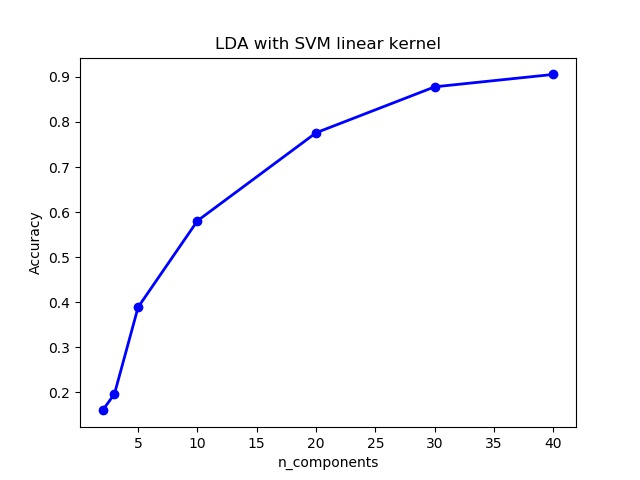
\includegraphics[width=6.5cm]{figure/LDA_linear.jpg}
%\caption{fig1}
}
\quad
\subfigure[metric accuracy comparison on LDA with RBF SVM]{
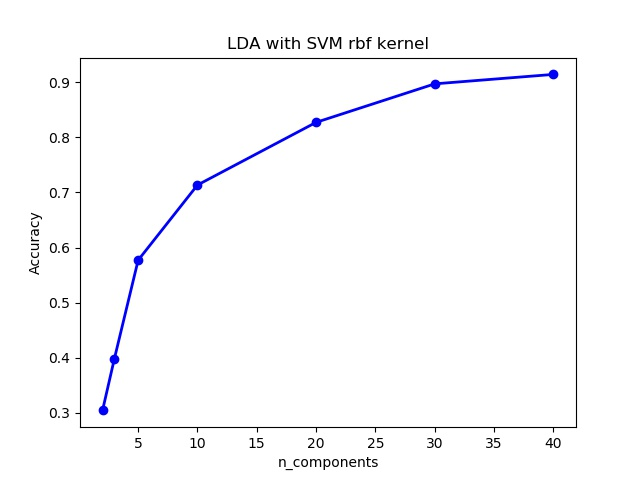
\includegraphics[width=6.5cm]{figure/LDA_rbf.jpg}
}
\caption{LDA-based model performance on linear kernel SVM and RBF kernel SVM}
\label{Fig3}
\end{figure}
\end{center}

\begin{center}
\begin{figure}[htbp]
\centering
\subfigure[Trainset 2D scatter with LDA]{
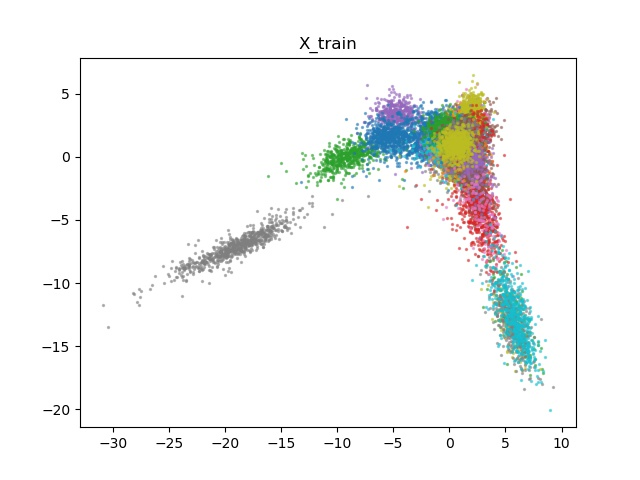
\includegraphics[width=6.5cm]{figure/X_train_scatter_2d_LDA.jpg}
%\caption{fig1}
}
\quad
\subfigure[Testset 2D scatter with LDA]{
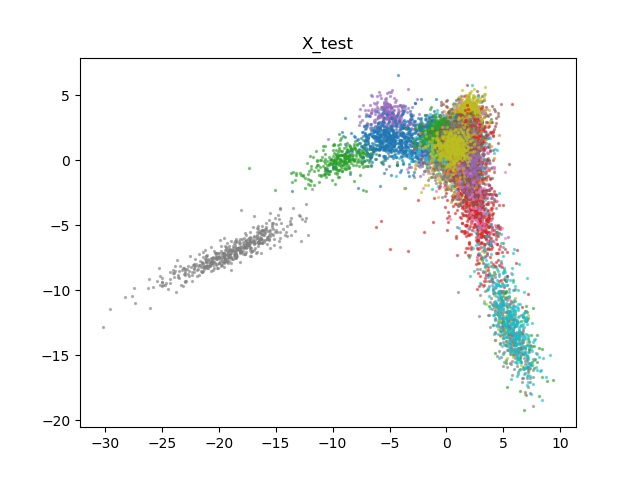
\includegraphics[width=6.5cm]{figure/X_test_scatter_2d_LDA.jpg}
}
\caption{Dataset 2-components scatter with LDA}
\label{Fig4}
\end{figure}
\end{center}

\begin{table}
	\centering
	\newcommand{\tabincell}[2]{\begin{tabular}{@{}#1@{}}#2\end{tabular}}
	\renewcommand\arraystretch{1.1}
	\caption{Comparison of AutoEncoder-based SVM and baslines in Classification Task}
	\label{baseline3}%
	\resizebox{\linewidth}{!}{
	\begin{tabular}{c|c|c|c|c}
		\hline
		Model &\multicolumn{2}{c|}{AutoEncoder+SVM}&\multicolumn{2}{c}{SVM}\\
		\hline
		{components number} & {Linear kernel(\%)} & {RBF kernel(\%)}& {Linear kernel(\%)} & {RBF kernel(\%)}\\
		\cline{2-5}
		\hline
		2   & 23.71 & 68.75 & 93.28 & 93.52\\
		\hline
		64   & 69.52 & 70.35 & 93.28 & 93.52\\
		\hline
		128   & 72.01 & 70.25 & 93.28 & 93.52\\
		\hline
		256   & 78.35 & 76.93 & 93.28 & 93.52\\
		\hline
		512   & 87.59 & 87.90 & 93.28 & 93.52\\
		\hline
		1024   & 91.42 & 91.95 & 93.28 & 93.52\\
		\hline
	\end{tabular}}
\end{table}

\subsubsection{AutoEncoder}
AutoEncoder is a unsupervised method to determine the essential dimensions of high-dimensional dataset, which can construct the complete dataset features with minimun loss, i.e. with encoder reducing the data dimension to `bottleneck' and decoder to restruct the data, we can get the origin sample data or get the minimun loss. In this section, we use AutoEncoder with MSE loss to get the low-dimensional feature and respectively combine linear SVM and RBF SVM to achieve the classification task. We adopt classifiction accuracy as metric in this section.

We summarize the experimental results of AutoEncoder-based model in Tab. \ref{baseline3} and Fig. \ref{Fig5}. As is shown, with the components number increases, models receive better performance especially for RBF kernel model. We can recognize that when we have less compoents, model with RBF SVM may receive a higher accuracy. AE with linear SVM and with RBF SVM respectively reach $91.42\%$ and $91.95\%$ in classification accuracy when components number comes to 1024.

We give the 2-components scattering figure of different kernel and dataset in Fig. \ref{Fig6}. We can find that some classes can't be linearly differed in 2-components, and we deem it's the reason why RBF SVM have better performance than linear one when we have less components.

\begin{center}
\begin{figure}[htbp]
\centering
\subfigure[metric accuracy comparison on AutoEncoder with linear SVM]{
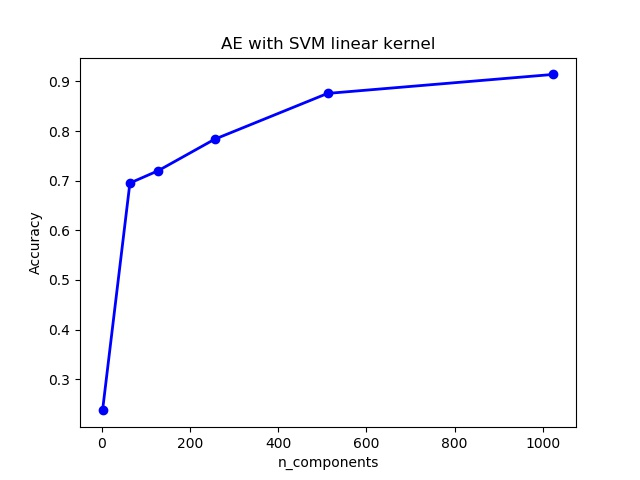
\includegraphics[width=6.5cm]{figure/AE_linear.jpg}
%\caption{fig1}
}
\quad
\subfigure[metric accuracy comparison on AutoEncoder with RBF SVM]{
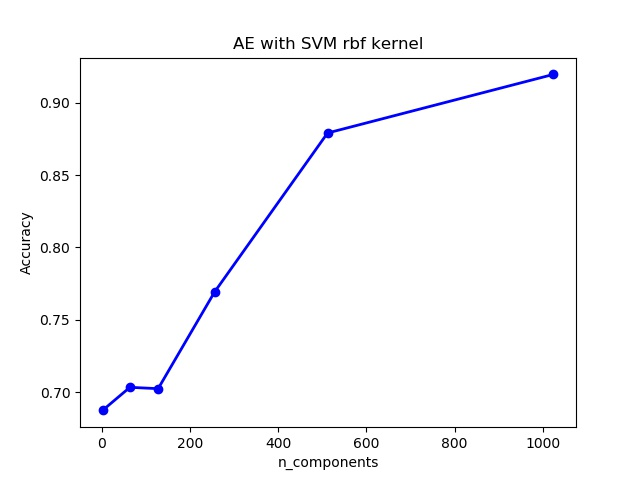
\includegraphics[width=6.5cm]{figure/AE_rbf.jpg}
}
\caption{AutoEncoder-based model performance on linear kernel SVM and RBF kernel SVM}
\label{Fig5}
\end{figure}
\end{center}

\begin{center}
\begin{figure}[htbp]
\centering
\subfigure[Trainset 2D scatter with AutoEncoder]{
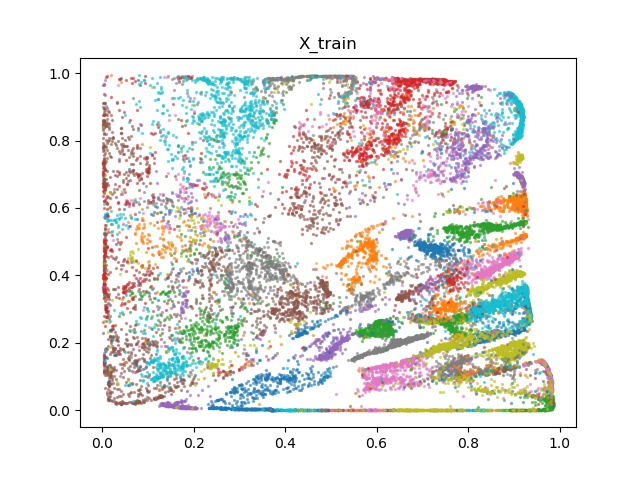
\includegraphics[width=6.5cm]{figure/X_train_scatter_2d_AE.jpg}
%\caption{fig1}
}
\quad
\subfigure[Testset 2D scatter with AutoEncoder]{
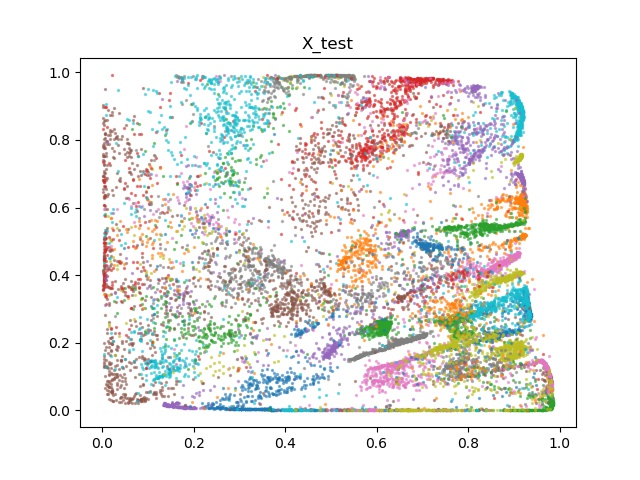
\includegraphics[width=6.5cm]{figure/X_test_scatter_2d_AE.jpg}
}
\caption{Dataset 2-components scatter with AutoEncoder}
\label{Fig6}
\end{figure}
\end{center}

\subsection{Feature Learning}
\subsubsection{t-SNE}

The technique t-SNE is a common method for high-dimensional data visualizing by giving each data point a location in a two or three-dimensional space. In this section, two experiment settings can derive from the rule: t-SNE used Barnes-Hut approximation to calculate gradient on dimension 2 and 3, and test parameter perplexity in $[10.0, 20.0, 30.0, 40.0, 50.0]$. 

tSNE with linear SVM receives its best performance $5.39\%$ when $perplexity=10.0$ while tSNE with RBF SVM reaches $5.95\%$ when $perplexity=10.0$. We deem the reason of low accuracy is that aim components number is not enough to extract efficient features to predict.

We also give the 2-components scattering result in Fig. \ref{Fig7}. tSNE enables different data clusters in low-dimension to be distant enough and the data points belonging to the same cluster to be close, which benefits classification. As is shown, we can differ various classes in 2D scattering. Besides, we can find with the parameter $perplexity$ increase, tSNE model can process more data.

\begin{figure}
\centering
\subfigure[Trainset 2D scatter with tSNE (perplexity=10.0)]{
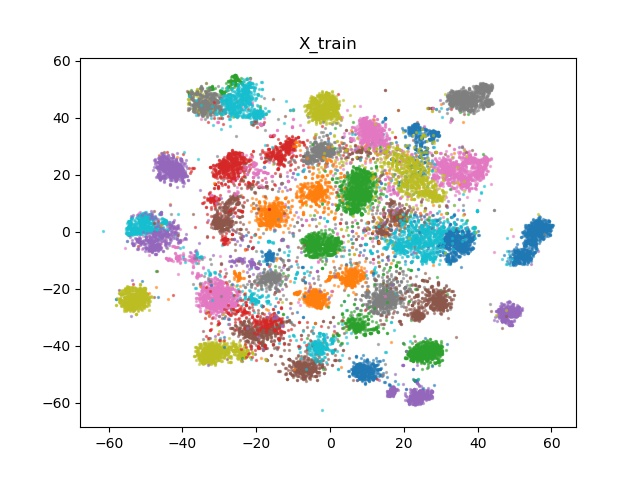
\includegraphics[width=2.9cm]{figure/X_train_scatter_2d_TSNE_10.jpg}
%\caption{fig1}
}
\quad
\subfigure[Trainset 2D scatter with tSNE (perplexity=20.0)]{
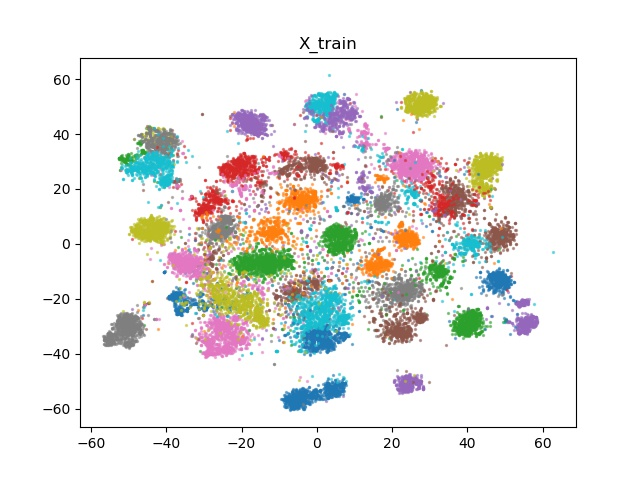
\includegraphics[width=2.9cm]{figure/X_train_scatter_2d_TSNE_20.jpg}
}
\quad
\subfigure[Trainset 2D scatter with tSNE (perplexity=30.0)]{
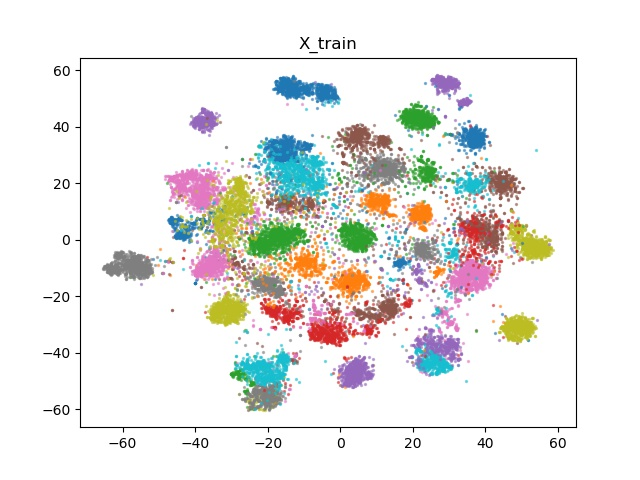
\includegraphics[width=2.9cm]{figure/X_train_scatter_2d_TSNE_30.jpg}
}
\quad
\subfigure[Trainset 2D scatter with tSNE (perplexity=40.0)]{
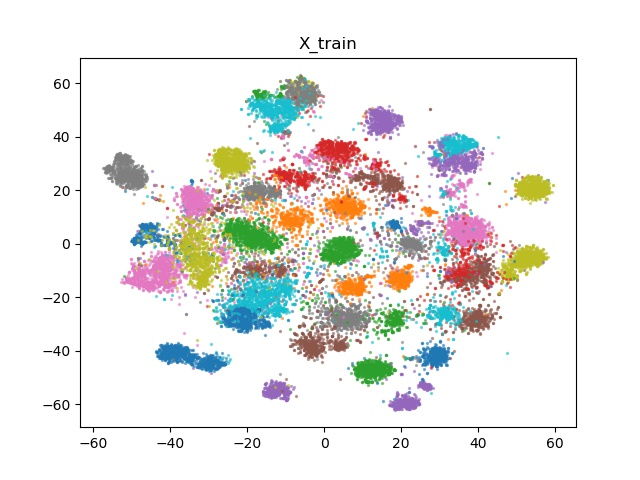
\includegraphics[width=2.9cm]{figure/X_train_scatter_2d_TSNE_40.jpg}
}
\quad
\subfigure[Trainset 2D scatter with tSNE (perplexity=50.0)]{
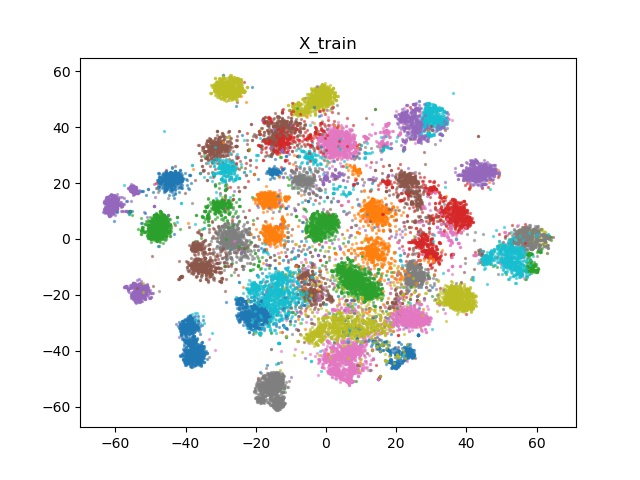
\includegraphics[width=2.9cm]{figure/X_train_scatter_2d_TSNE_50.jpg}
}
\quad
\subfigure[Testset 2D scatter with tSNE (perplexity=10.0)]{
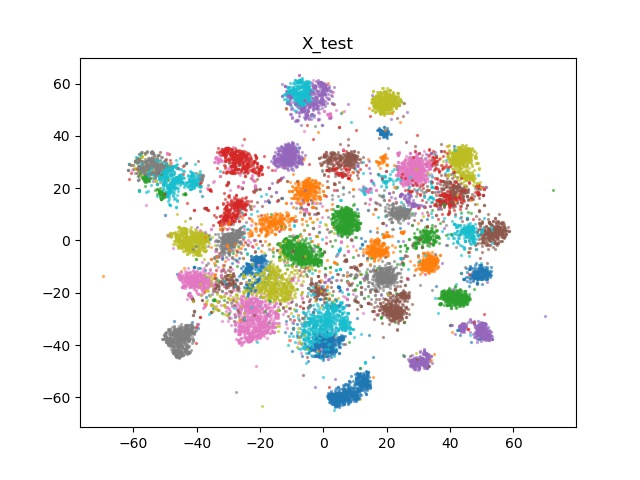
\includegraphics[width=2.9cm]{figure/X_test_scatter_2d_TSNE_10.jpg}
}
\quad
\subfigure[Trainset 2D scatter with tSNE (perplexity=20.0)]{
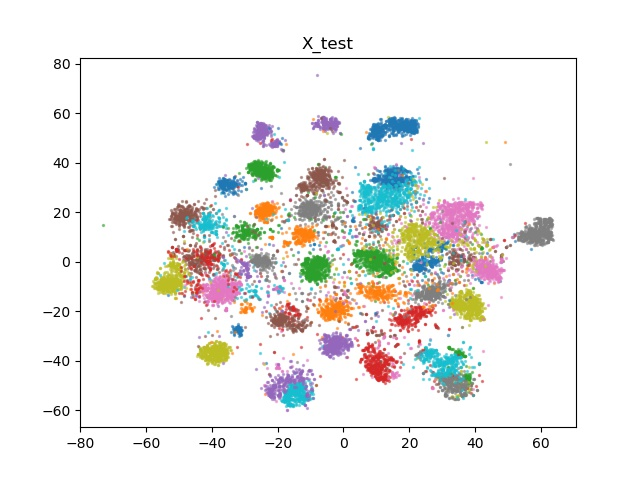
\includegraphics[width=2.9cm]{figure/X_test_scatter_2d_TSNE_20.jpg}
}
\quad
\subfigure[Testset 2D scatter with tSNE (perplexity=30.0)]{
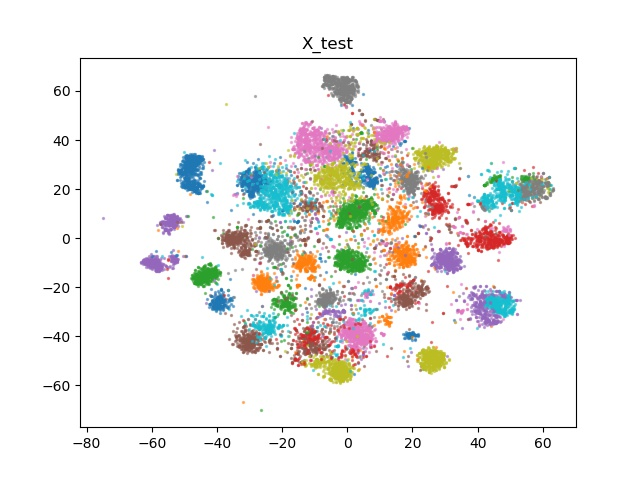
\includegraphics[width=2.9cm]{figure/X_test_scatter_2d_TSNE_30.jpg}
}
\quad
\subfigure[Trainset 2D scatter with tSNE (perplexity=40.0)]{
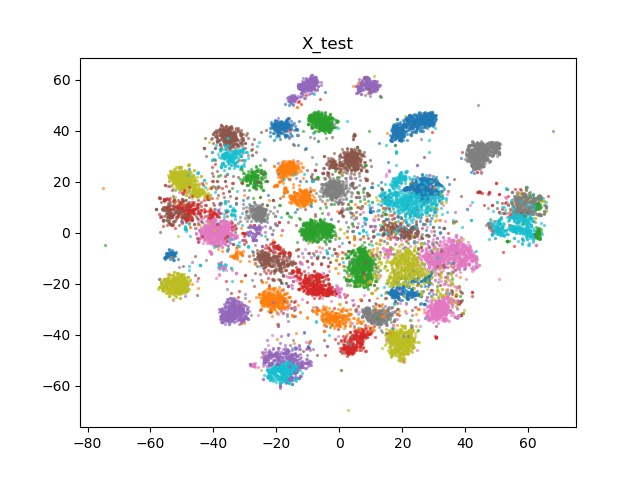
\includegraphics[width=2.9cm]{figure/X_test_scatter_2d_TSNE_40.jpg}
}
\quad
\subfigure[Testset 2D scatter with tSNE (perplexity=50.0)]{
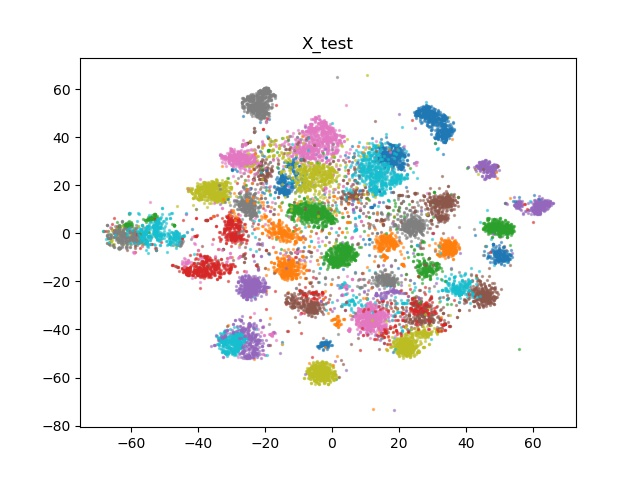
\includegraphics[width=2.9cm]{figure/X_test_scatter_2d_TSNE_50.jpg}
}
\caption{Dataset 2D scatter with tSNE on perplexity of $\{10.0,20.0,30.0,40.0,50.0\}$}
\label{Fig7}
\end{figure}

\subsubsection{LLE}
Locally Linear Embedding (LLE) is a feature learning mathod which tried to keep the linear relation between neighbor samples. In this section, we respectively use 4, 8 and 16 neighbors to rule the experiments and our aim components range is $[2, 3, 50, 100, 500, 1000, 2000]$.

We summarize the experimental results of AutoEncoder-based model in Tab. \ref{baseline3} and Fig. \ref{Fig5}. We can find if we maintain more neighbor relations and more aim components, we can get better performance, i.e. LLE with Linear SVM receives $90.60\%$ and LLE with RBF SVM receives $90.18\%$. Performance of LLE is satisfiying beacause original features may have simple structure and the data is randomly scatering in the high-dimension space.

We also give the 2-components scattering result in Fig. \ref{Fig7}. When we use 4 neighbors to reconstruct the sample, we can find its poor performance. For data can be regarded as manifold structure, LLE performs while when we give the proper neighbors' number.

\section{Conclusion}
In this project, we evaluate different dimension reduction techniques by measuring their classification performance when combined with SVM model. In this Section, we want to give our perspectives on drawbacks and merits of these dimension reduction method. Importantly, we'll conclude the situations to use these methods.

\bibliography{bibfile.bib}
\end{document}